%!TEX program = xelatex
% 完整编译: xelatex -> biber/bibtex -> xelatex -> xelatex
\documentclass[lang=cn,a4paper,newtx,bibend=bibtex]{elegantpaper}

\title{Problems of Chapter 4}
\author{张志心 \ 混合2106}

\date{\zhdate{2023/12/3}}

% \qedhere to make the square straight after

\usepackage{array}
\usepackage{tcolorbox}
\usepackage{tikz}
\usepackage{pgfplots}
\usepackage{float}

\newtcolorbox{prob}[1][]{
  colframe=gray,
  colback=white,
  boxrule=1.5pt, % 控制外边框线的宽度
  sharp corners, % 使用直角边框
  fonttitle=\bfseries,
  title=#1
}

\newcommand{\ccr}[1]{\makecell{{\color{#1}\rule{1cm}{1cm}}}}
\pgfplotsset{compat=1.17}

\addbibresource[location=local]{reference.bib}

\begin{document}

\maketitle

\section{Theoretical questions}

\begin{prob}[4.4.1-\textrm{I}.]
  Convert the decimal integer 477 to a normalized FPN with $\beta = 2$.
\end{prob}

\begin{solution}
  $477 = (111011101)_2 = (1.11011101)_2\times 2^8$
\end{solution}



\begin{prob}[4.4.1-\textrm{II}.]
  Convert the decimal fraction 3/5 to a normalized FPN with $\beta = 2$.
\end{prob}

\begin{solution} 
 $\frac35 = (0.\dot{1}00\dot{1})_2 = (1.\dot{0}01\dot{1})_2 \times 2^{-1}$
\end{solution}

\begin{prob}[4.4.1-\textrm{III}.]
  Let $x = \beta^e, e\in \mathbb{Z}, L < e < U$ be a normalized FPN in $\mathbb{F}$
  and $x_L, x_R\in \mathbb{F}$ are the two normalized FPNs adjacent to $x$ such that
  $x_L < x < x_R$. Prove $x_R - x = \beta(x - x_L)$.
\end{prob}

\begin{proof}
  根据题意 $x = 1.0 \times \beta^e$,
  $x_R = (1 + \beta^{-p + 1})\times \beta^e, x_L = \left[\sum_{i = 0}^{p-1} (\beta - 1)\beta^{-i}\right]\times\beta^{e- 1} = (1- \beta^{-p})\times \beta^e$。
  所以 $x_R - x = \beta^{e-p+1}, x-x_L = \beta^{e-p}$, $x_R - x = \beta(x - x_L)$。
\end{proof}

\begin{prob}[4.4.1-\textrm{IV}.]
  By reusing your result if \textrm{II}, find out the two normalized FPNs adjacent
  to $x = 3/5$ under the IEEE 754 single-precision protocol. What is $\text{fl}(x)$ and 
  the relative roundoff error?
\end{prob}

\begin{solution}
  在 IEEE 754 单精度浮点数系统下,尾数为 23 位。所以:
  \[x_L = (1.00110011001100110011001)_2 \times 2^{-1}, x_R = (1.00110011001100110011010)_2\times 2^{-1}\]
  显然 $x_R - x < x - x_L$,所以 $\text{fl}(x) = x_R$,相对误差 $E_{rel}(x_R) = \dfrac{|x_R - x|}{|x|} = \dfrac{(0.\dot{0}11\dot{0})_2\times 2^{-23}}{3/5} = \dfrac{2}{3}\times 2^{-23}$。
\end{solution}

\begin{prob}[4.4.1-\textrm{V}.]
  If the IEEE 754 single-precision protocol did not round
  off numbers to the nearest, but simply dropped excess
  bits, what would the unit roundoff be?
\end{prob}

\begin{solution}
  设 $x = (m_x + \beta^{1-p} - \epsilon) \times \beta^n$,其中 $0 < \epsilon < \beta^{-p+1}$,则 $\text{fl}(x) = m_x \times \beta^n$。

  \[\delta = \left|\dfrac{\text{fl}(x) - x}{x}\right| = \dfrac{\beta^{1-p}-\epsilon}{m_x + \beta^{1-p}-\epsilon} \rightarrow \dfrac{\beta^{1-p}}{m_x + \beta^{1-p}} (\epsilon \rightarrow 0^+)\]

  又因为 $1\le m_x < \beta$, 所以有 $\delta < \beta^{1-p} = \epsilon_M (= 2^{-23})$ 成立,所以舍入单位 $\epsilon_u = \epsilon_M$。
\end{solution}


\begin{prob}[4.4.1-\textrm{VI}.]
  How many bits of precision are lost in the subtraction
  $1-\cos x$ when $x = \frac14$?
\end{prob}

\begin{solution}
  $\cos \frac14 = 0.9689\cdots, 1 - \cos \frac14 = 0.0310\cdots \in (2^{-6}, 2^{-5})$,因此损失了 6 位的精度。
\end{solution}

\begin{prob}[4.4.1-\textrm{VII}.]
  Suggest at least two ways to compute $1 - \cos x$ to avoid
  catastrophic cancellation caused by subtraction.
\end{prob}

\begin{solution}
  为了避免减法运算带来的巨量消失,考虑将减法转化为别的四则运算。
  \begin{enumerate}
    \item $1-\cos x = \begin{cases} \text{fl}(1-\text{fl}(\cos x)) & \cos x < 0 \\ \text{fl}\left(\dfrac{\text{fl}(\text{fl}(\sin x))^2}{\text{fl}(1 + \text{fl}(\cos x))}\right) & \cos \ge 0\end{cases}$
    \item $1 - \cos x = 2\text{fl}(\sin (\frac{x}2))^2$
    \item $1 - \cos x = \text{fl}[\text{fl}(\frac{x^2}{2!}) - \text{fl}(\frac{x^4}{4!}) + \text{fl}(\frac{x^6}{6!}) - \cdots ] = \text{fl}\left[\sum_{k = 1}^{M} \text{fl}\left((-1)^{k+1}\frac{x^{2k}}{(2k)!}\right)\right]$,这里 $M$ 可以取一个足够大的整数,使得计算的相对误差在可接受范围内。
  \end{enumerate}
\end{solution}

\begin{prob}[4.4.1-\textrm{VIII}.]
  What are the condition numbers of the following functions?
  Where are they large?
  \begin{itemize}
    \item $(x-1)^{\alpha}$
    \item $\ln x$
    \item $e^x$
    \item $\arccos x$
  \end{itemize}
\end{prob}

\begin{solution} ~~%<br>

  \begin{itemize}
    \item $\text{Cond}_f (x) = \begin{cases} \left| \dfrac{x \mathrm{d} (x - 1)^{\alpha - 1}}{(x - 1)^{\alpha}} \right| = \left|\dfrac{\alpha x}{x - 1}\right| & \alpha \neq 0 \\ 
            0 & \alpha = 0\end{cases}$
          ,$\lim_{x\to 1}\text{Cond}_f(x) = \infty (\alpha \neq 0)$;
    \item $\text{Cond}_f (x) = \left|\dfrac{x \cdot \frac1x}{\ln x}\right| = \dfrac{1}{|\ln x|}$, $\lim_{x\to 1} \text{Cond}_f(x) = \infty$;
    \item $\text{Cond}_f (x) = \left|\dfrac{x\cdot e^x}{e^x}\right| = |x|$,$\lim_{x \to \infty} \text{Cond}_f(x) = \infty$;
    \item $\text{Cond}_f (x) = \left|\dfrac{x\cdot \frac{-1}{\sqrt{1-x^2}}}{\arccos x}\right| = \left|\dfrac{x}{\sqrt{1-x^2}\arccos x}\right|$,$\lim_{x\to \pm 1}\text{Cond}_f(x) = \infty$。
  \end{itemize}
\end{solution}

\begin{prob}[4.4.1-\textrm{IX}.]
  Consider the function $f(x) = 1 - e^{-x}$ for $x \in [0, 1]$.
  \begin{itemize}
    \item Show that $\text{cond}_f(x) \le 1$ for $x \in [0, 1]$.
    \item Let $A$ be the algorithm that evaluates $f(x)$ for
    the machine nuumber $x \in F$. Assume that the exponential 
    function is computed with relative error
    within machine roundoff. Estimate $\text{cond}_A(x)$ for
    $x \in [0, 1]$.
    \item Plot $\text{cond}_f(x)$ and the estimated upper bound of
    $\text{cond}_A(x)$ as a function of $x$ on $[0, 1]$. Discuss your 
    results.
  \end{itemize}
\end{prob}

\begin{solution} ~~%<br>

  \begin{itemize}
    \item $\text{Cond}_f(x) = \left|\frac{xe^{-x}}{1-e^{-x}}\right|  = \frac{x}{1 - e^x}, \forall x \in [0, 1]$,因为 $(\frac{x}{1-e^{-x}})' = \frac{(1 - x - e^{-x})e^{-x}}{(1- e^{-x})^2}\le 0 (x \in [0, 1])$,
          并且在 $x = 0$ 处 $\lim_{x\to 0} \text{Cond}_f(x) = 1$,所以 $\text{Cond}_f (x) \le 1, \text{ for } x\in [0, 1]$;
    \item $f_A(x) = \text{fl}(1 - \text{fl}(e^{-x})) = (1 - e^{-x}(1 + \delta_1))(1 + \delta_2) \simeq (1 - e^{-x})(1 + \delta_2 + \delta_1\frac{e^{-x}}{1 - e^{-x}})$,
   
    因此有 $f_A(x) = f(x)(1 + \delta(x)), |\delta(x)| = \left|\delta_2 + \delta_1\frac{e^{-x}}{1 - e^{-x}}\right|\le |\frac{\delta_2 + (\delta_1 - \delta_2)e^{-x}}{1 - e^{-x}}| \le \frac{\epsilon_u}{1 - e^{-x}}$,
    
    $\text{Cond}_A(x) \le \frac{1}{(1- e^{-x})\text{Cond}_f(x)} = \frac1{xe^{-x}}$;
    \item 如下图所示,$\text{Cond}_f(x), \text{upper bound of Cond}_A(x)$ 均在 $x\to 0$ 最大,且 $\text{Cond}_A > \text{Cond}_f$。
    \begin{center}
    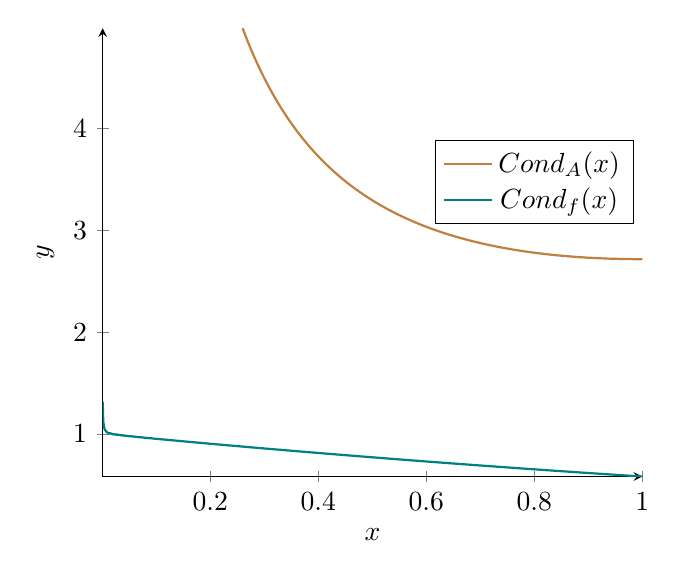
\begin{tikzpicture}
      \begin{axis}[
        xlabel={$x$},
        ylabel={$y$},
        domain=0:1,
        restrict y to domain=0:5,
        samples=1000,
        axis lines=left,
        legend style={at={(0.8,0.75)},anchor=north},
        ]
        
        \addplot[brown, thick, domain=0.001:1] {1/(x*exp(-x))};
        \addlegendentry{$\text{Cond}_A(x)$}

        \addplot[teal, thick, domain=0.001:1] {(x*exp(-x))/(1-exp(-x))};
        \addlegendentry{$\text{Cond}_f(x)$}
      \end{axis}
    \end{tikzpicture}
  \end{center}
  \end{itemize}
\end{solution}

\begin{prob}[4.4.1-\textrm{X}.]
  Prove Lemma 4.68. Base on the 2-norm, the condition number of a nonsingular square
  matrix $A$ is
  \[\text{cond} A := \|A\|_2\|A^{-1}\|_2 = \dfrac{\sigma_{max}}{\sigma_{min}}.\]
  where $\sigma_{max}$ and $\sigma_{min}$ are respectively the largest and the
  smallest singular values of $A$. If $A$ is also normal, we have, 
  \[\text{cond}_2 A = \dfrac{\lambda_{max}}{\lambda_{min}}\]
  where $\lambda_{max}$ and $\lambda_{min}$ are eigenvalues of $A$ with the largest
  and the smallest moduli, respectively. Furthermore, if $A$ is unitary, we have 
  $\text{cond}_2 A = 1$.
\end{prob}

\begin{proof}
  \begin{equation*}
    \begin{aligned}
      \| A \|_2^2 &= \sup_{\| x\|_2 =1} \| Ax\|_2^2 = \sup_{\|x\|_2 = 1} (Ax)^T(Ax)
       = \sup_{\|x\|_2 = 1} x^TA^TAx = \sup_{\|x\|_2 = 1}x^TP^T\Lambda Px = \sup_{\| Px\|_2 = 1}(Px)^T\Lambda (Px) = \lambda_{max} \\
       \| A^{-1} \|_2^2 &= \sup_{\|x\|_2 = 1} \| A^{-1}x\|_2^2 = \cdots = \sup_{\|Px\|_2 = 1} (Px)^T \Lambda^{-1} (Px) = \lambda_{min}^{-1} \\
       \Rightarrow \text{Cond} &(A) = \| A\|_2 \|A^{-1}\|_2 = \sqrt{\frac{\lambda_{max}}{\lambda_{min}}} = \frac{\sigma_{max}}{\sigma_{min}}
    \end{aligned}
  \end{equation*}
\end{proof}

\begin{prob}[4.4.1-\textrm{XI}.]
  The math problem of root finding for a polynomial
  \[q(x) = \sum_{i = 0}^n a_i x^i, \quad\quad a_n = 1, a_0\neq 0, a_i \in \mathbb{R}\]
  can be considered as a vector function $f : \mathbb{R}^n \to \mathbb{C}$:
  \[r = f(a_0, a_1, \cdots, a_{n-1}).\]
  Derive the componentwise condition number of $f$ based
  on the $1$-norm. For the Wilkinson example, compute
  your condition number, and compare your result with that 
  in the Wilkinson Example. What does the comparison tell you?
\end{prob}

\begin{solution}
  $\text{Cond}_f(\mathbf{a}) = \max_{j}\left|\dfrac{a_j\frac{\partial f}{\partial a_j}}{f(a)}\right|$,
  
  $\dfrac{\partial f}{\partial a_j}(\mathbf{a}) = \lim_{\epsilon\to 0} \frac{-\epsilon \frac{r^j}{q'(r)}}{\epsilon} = -\dfrac{r^j}{q'(r)}, r = f(a)$, 即 $q(x)$ 的根。
  
  所以 $\text{Cond}_f(\mathbf{a}) = \max_j \left|\dfrac{a_jr^{j-1}}{q'(r)}\right|$,

  对于 Wilkinson 例子即 $q(x) = \prod_{i = 1}^p(x - i)$,当 $p$ 足够大时,
  对于 $q(x)$ 最大根 $p$,
  \[\text{Cond}_f(\mathbf{a}) = \max_j \left|\dfrac{a_j p^{j-1}}{(p-1)!}\right| = \dfrac{\max_j |a_j p^{j-1}|}{(p-1)!}\]
  
  其中 $a_j$ 是 $\prod_{i = 1}^{p}(x- i)$ 的 $j$ 次项系数,
  注意到 $|a_{p-1}| = \frac{p(p-1)}{2}$,因此 $\text{Cond}_f(x)$ 至少和 $\dfrac{p^p}{2(p-2)!}$ 同阶。

  所以 $n\to \infty$ 的时候,$\text{Cond}_f(\mathbf{a})\to \infty$。可以看出求得高阶多项式的数值根是很困难的。
\end{solution}

\begin{prob}[4.4.1-\textrm{XII}.]
  Suppose the division of two FPNs is calculated in a register 
  of precision $2p$. Give an example that contradicts
  the conclusion of the model of machine arithmetic.
\end{prob}

\begin{solution}
  取 FPN 系统 $\beta = 2, p = 2, L = -1, U = 1$,考虑 $a = 1,b = \frac32$ 两个数在该系统中,
  则 $\text{fl}(\frac{a}b) = \text{fl}((1.010)_2\times 2^{-1}) = (1.0)_2\times 2^{-1}$,
  相对误差为 $\frac{-0.5 + \frac23}{\frac23} = 2^{-2} = \epsilon_u$,矛盾。
\end{solution}

\begin{prob}[4.4.1-\textrm{XIII}.]
  If the bisection method is used in single precision FPNs
  of IEEE 754 starting with the interval $[128, 129]$, can
  we compute the root with absolute accuracy $< 10^{−6}$?
  Why?
\end{prob}

\begin{solution}
  在单精度系统下 $\epsilon_u = \frac12\epsilon_M = 2^{-24}$,根的绝对误差最大为 $129 \times 2^{-24} \approx 7.69 \times 10^{-6} > 10^{-6}$。不能。
\end{solution}

\begin{prob}[4.4.1-\textrm{XIV}.]
  In fitting a curve by cubic splines, one gets inaccurate
  results when the distance between two adjacent points
  is much smaller than those of other adjacent pairs. Use
  the condition number of a matrix to explain this phenomenon.
\end{prob}

\begin{solution}
  对于在 $[x_i, x_{i+1}]$ 上的样条函数 $s(x)$,求解时需根据 $s(x_i), s(x_{i+1}), s'(x_i), s'(x_{i+1})$ 的值列出
  方程进行求解,方程的系数矩阵如下:

  \begin{equation*}
    \begin{bmatrix}
      x_i^3 & x_i^2  & x_i & 1 \\
      x_{i+1}^3 & x_{i+1}^2 & x_{i+1} & 1 \\
      3x_i^2 & 2x_i & 1 & 0 \\
      3x_{i + 1}^2 & 2x_{i+1} & 1 & 0
    \end{bmatrix}
  \end{equation*}


  在 $|x_{i+1}-x_i|$ 很小的情况下,上述矩阵的$1,2$两行和$3,4$两行的值十分接近,
  因此上述矩阵是一个病态矩阵,其最小特征值接近于 $0$,所以求解该样条函数的准确性很差。

\end{solution}

\section{Programming assignments}

\subsection{A}

计算以下三个函数在 $[0.99, 1.01]$ 上 101 个等距点上的函数值并作图。
注意这三个函数在理论上是完全相同的。观察结果并解释原因。

代码实现:见 \lstinline{Problem-A.cpp}

运行结果:见 \lstinline{res/Output_A.csv}

将三个函数的图像绘制如下:

\begin{figure}[H]
  \centering
  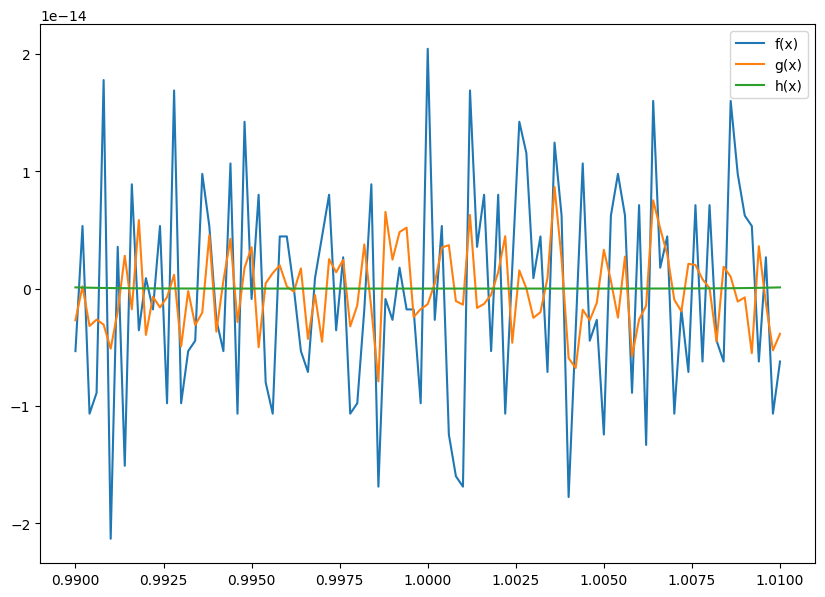
\includegraphics[width=0.8\linewidth]{output_A.png} 
  \caption{$f(x), g(x), h(x)$ 对比图}
\end{figure}

\[
  f(x) = x^7 - 8x^7 + 28x^6 - 56x^5 + 70x^4 - 56x^3 + 28x^2 -8x + 1
\]
\[
  g(x) = (((((((x-8)x+28)x-56)x+70)x-56)x+28)x-8)x + 1
\]
\[
  h(x) = (x - 1)^8
\]

 由图像,$h$ 的精确度比 $f,g$ 显著高。$f$ 是振荡最厉害的,最不精确。
 
 三个函数的条件数都是 $|\frac{8x}{x-1}|$,
 在 $x\to 1$ 的条件数区域正无穷,在 $1$ 附近计算的函数值容易不精确。

 然而 $h(x)$ 的精确度比另外两个高很多,这是因为 $f(x),g(x)$ 的计算方法
 的最后一步,都是进行 $\phi(x) + 1$, 其中 $\phi(x) = f(x) - 1$ 非常接近
  $-1$($f(x)$ 的绝对值在 $[10^{-30}, 10^{-16}]$ 之间数量级接近甚至小于 $\epsilon_u$),
  因此进行最后一次计算的时候,将会导致巨量消失,导致有效位被舍入。
而 $h(x)$ 只在最开始进行了一次减法运算 $x-1$ 只会损失一部分精度,且 $x-1$ 的数量级
高于 $\epsilon_u$,之后 $h(x)$ 只进行乘法运算,精度损失很小。
而 $f(x)$ 和 $g(x)$ 则进行了大量的加减运算,相近的数运算带来了很多的精度损失。

 $g(x)$ 利用相比 $f(x)$,使用了秦九韶法,大大减少了乘除法的计算次数,提高了精确度。



\subsection{B}

代码实现:见 \lstinline{Problem-B.cpp}

考虑正则 FPN 系统 $\mathbb{F}$ : $\beta = 2, p = 3, L = -1, U = 1$。

\begin{enumerate}
\item $\text{UFL}(\mathbb{F}) = \beta^L = 0.5$

      $\text{OFL}(\mathbb{F}) = \beta^U(\beta - \beta^{1-p}) = 3.5$;
\item $\mathbb{F}$ 中所有浮点数一共 25 个:
\begin{lstlisting}
  -3.5,-3,-2.5,-2,-1.75,-1.5,-1.25,-1,-0.875,-0.75,-0.625,
  -0.5,0,0.5,0.625,0.75,0.875,1,1.25,1.5,1.75,2,2.5,3,3.5
\end{lstlisting}
与讲义中关于 $\#\mathbb{F}$ 的推论相符合:$\#\mathbb{F} = 2^p(U-L+1)+1 = 8\times 3 + 1 = 25$。
\item 在数轴上画出 $\mathbb{F}$ 如下:
\begin{figure}[H]
  \centering
  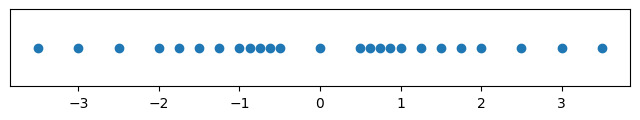
\includegraphics[width=0.8\linewidth]{output_B1.png}
\end{figure}
\item $\mathbb{F}$ 中所有非正则浮点数一共 6 个:
\begin{lstlisting}
  -0.375,-0.25,-0.125,0.125,0.25,0.375
\end{lstlisting}
\item 在数轴上画出扩展的 $\mathbb{F}$ 如下:
\begin{figure}[H]
  \centering
  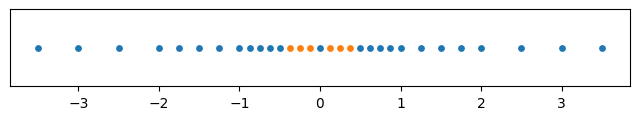
\includegraphics[width=0.8\linewidth]{output_B2.png}
\end{figure}
\end{enumerate}

\end{document}